\documentclass[10pt]{article}
\usepackage{itcep, stmaryrd, tikz, pgflibraryplotmarks, multicol}
\usepackage[margin=1in, nohead, pdftex]{geometry}
\usepackage{MnSymbol,wasysym}
\usepackage{hyperref}

\topmargin -0.2in
\pagestyle{empty}
\singlespacing
\let\oldhat\hat
\renewcommand{\vec}[1]{\mathbf{#1}}
\renewcommand{\hat}[1]{\oldhat{\mathbf{#1}}}

\definecolor{light-gray}{gray}{0.95}
\newcommand{\code}[1]{\colorbox{light-gray}{\texttt{#1}}}

\newcommand{\headerclass}{\code{<run>:\textbackslash the\textbackslash world} Machine Learning Camp}
\newcommand{\headersection}{Day 2: Exploring Data with Algorithms}
\newcommand{\headertitle}{Classification using Decision Trees}

\def\C{\mathbb{C}}
\def\R{\mathbb{R}}
\parindent 0ex
\begin{document}
%==================================================================================================================================================
\headerclass\xspace \hspace{\stretch{1}} \headersection\\
\begin{center}{ \large \textbf{\headertitle} }\end{center}
%==================================================================================================================================================



Decision trees are another way of classifying! The cool thing about decision trees is that you can use it for many types of problems, including ones with continuous variables (like our points $(x,y)$, or height, or time, or price) and problems with categorical variables (categories like yes/no, buy/hold/sell, fitted/loose, etc). 
	Decision trees usually involved drawing out a tree, and at each branch you make a decision. When you play Twenty Questions you are using a decision tree.
\bigskip
\begin{center}
Big idea: Pick the right questions to separate the groups
\end{center}
\bigskip
Fake data first:
	Here is some fake data, designed to be nice. Can you ask a question about one variable (just the $x$ coordinate, or just the $y$ coordinate) that would allow you to decide if you should have a black dot or a white dot?

 
\begin{center}
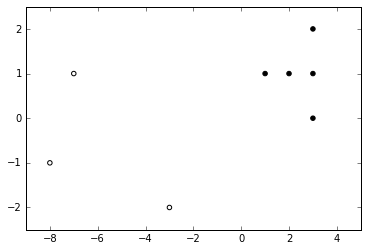
\includegraphics{TwoClusters.png}
\end{center}

Talk with your neighbor -- do you agree?


\pagebreak

Go backward this time: I'll give you a decision tree, and you draw a set of points that agrees with the decision tree rules.
\begin{center}
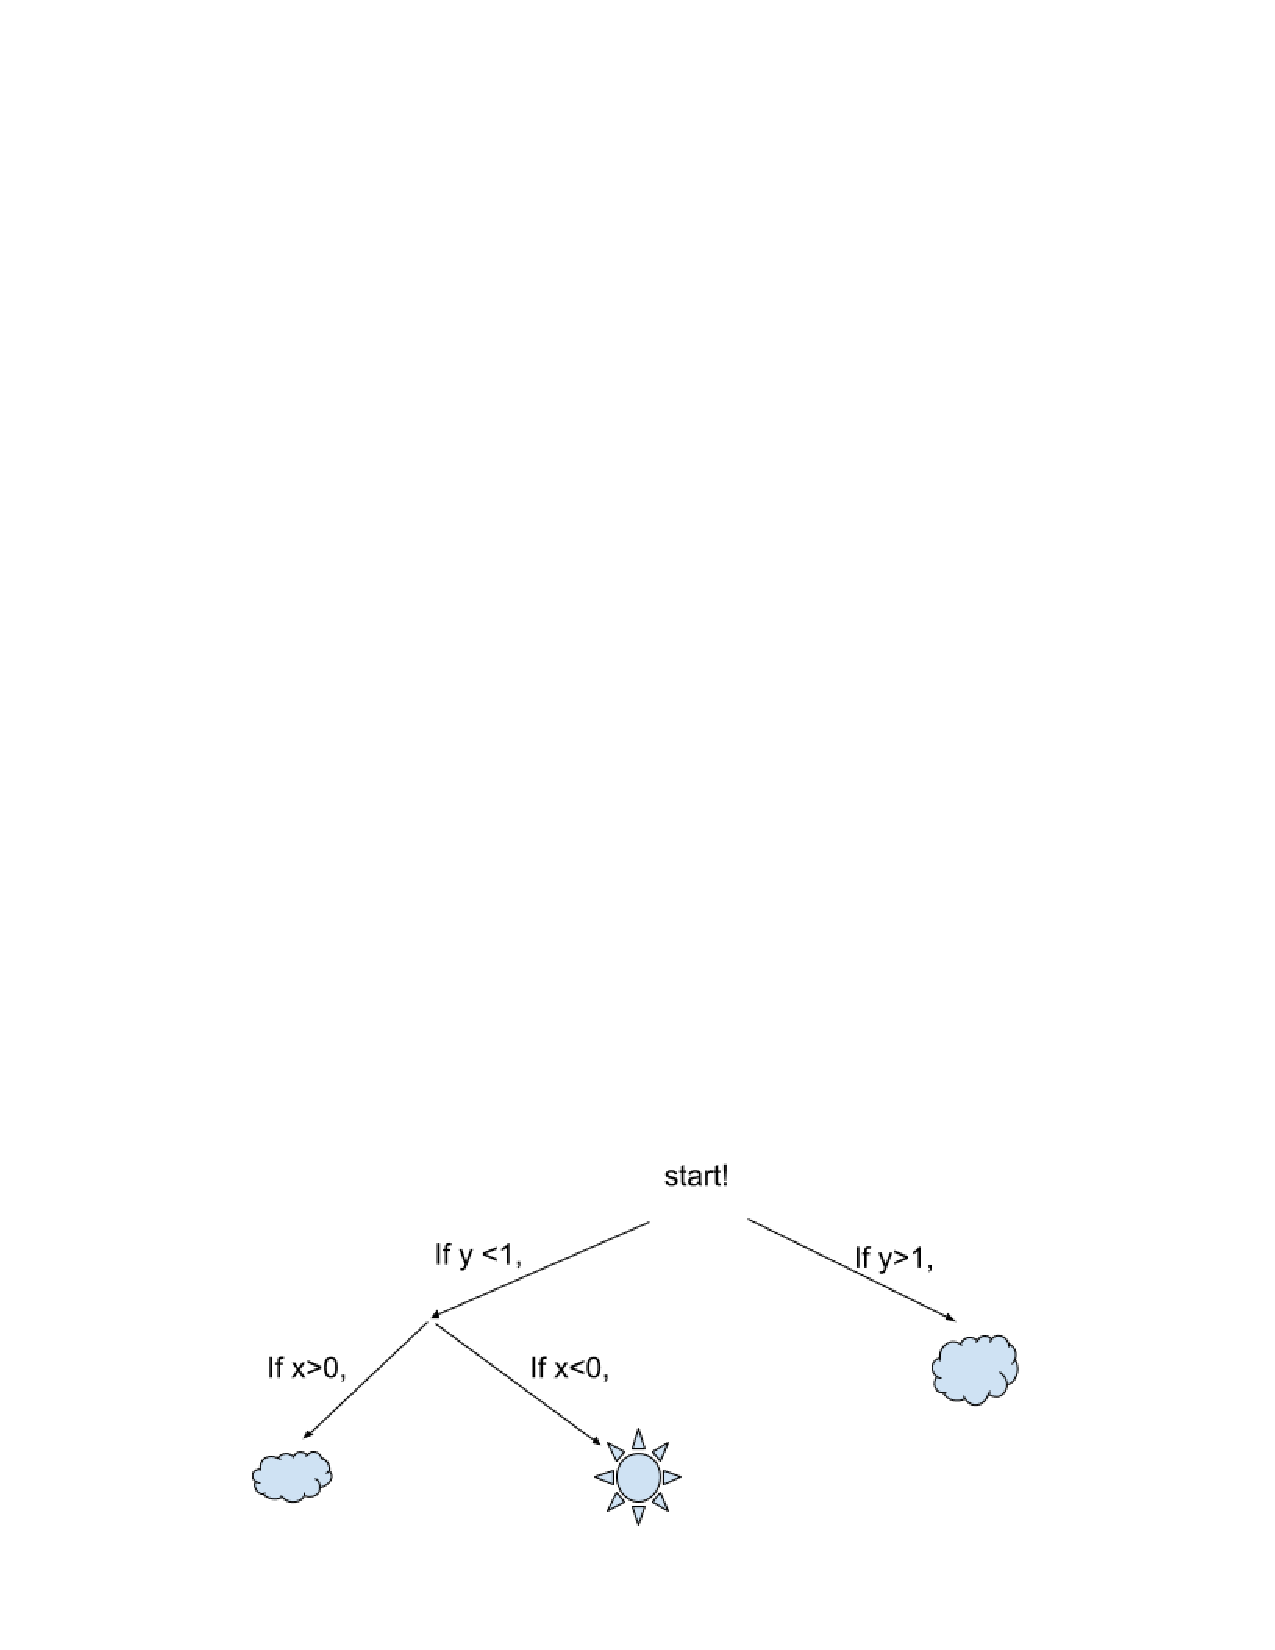
\includegraphics{SunMoonDT.pdf}
\end{center}

Draw the set of points $(x,y)$ that should be sunny and the set of points that should be cloudy according to this decision tree:
\vfill

\pagebreak


The sun and cloud symbols above are fun but also point to a set of examples people have used in textbooks about machine learning and data mining (another set of words for learning from data). Here's a version of this classic example:
\textit{You are trying to figure out if your little sister's soccer game will happen today. Last year, you know the following happened:}

\begin{center}

\begin{tabular}{|c|c|c|c|}
\hline
Temperature &
Rain &
Humidity &
Play \\
\hline
90 &
no &
high &
no \\
73&
no&
low&
yes \\
81&
yes&
high&
no \\
67&
no&
high&
yes\\
72&
yes&
high&
yes\\
77&
no&
low&
yes\\
96 &
no&
low&
no\\
81&
yes&
high&
no\\
58&
yes&
high&
yes\\
72&
no&
medium&
yes\\
\hline
\end{tabular}
\end{center}

This weekend, you don't think it will rain but it will be 90 degrees and 76 percent humidity. Do you think the game will happen? What about if it will rain but it will be 70 degrees with low humidity?

\vfill
Here there are two outcomes (play/don't play) but three variables. Hard to draw a picture. Could you make a decision tree that works pretty well by trial and error? Use this as scratch paper and try making a decision tree:
\vfill
\pagebreak


\begin{center}
Deciding on the decision tree
\end{center}
Back to the usual problem: what is the best decision tree? Depends on your definition of ``best,'' of course! Two ways are really common: Gini index/Gini impurity\footnote{Gini impurity measures how likely a mistake is if you stopped at a branch and just randomly picked some outcome from that division. Ask if you want to know more.}, and information gain. We?ll concentrate on information gain in this camp.


Information gain uses the concept of information entropy, how much information is contained in a set of data (!). Yes, this entropy is also the measure of disorder in the universe! Entropy is a number between zero and one. You can think of it as a measure of disorder or of uncertainty. For instance, 
\begin{itemize}
\item if you have a two-headed coin, there is no uncertainty about the outcome! Its entropy is zero.
\item If you have a fair coin, heads and tails are equally likely outcomes. There is maximum uncertainty. The entropy of the outcome is one.
\item  If you have an unfair coin that comes up heads $\frac{3}{4}$ of the time, there is less uncertainty! You?d want to bet on heads, right? The entropy of the outcome is about 0.81128. 
Can you check this?
\end{itemize}


Information gain is about the change in entropy as you make branches in the decision tree.
We?ll implement entropy calculations in Excel. They are kind of a pain to do. You will be very happy to move to Python?.


Let?s look at entropy and information gain. 
You?re doing a classification problem, so you want to classify outcomes as ?yes? or ?no?, for instance. Let $p_1$ be the fraction of ?yes? outcomes and $p_2$ the fraction of ?no? outcomes.
The entropy of the whole set, or information content, is $-p1log2 p1- p2log2 p2$.
If only one outcome happens (only ?yes? or only ?no? in our example) we say the entropy is zero. 

Question 1: For the soccer game example, what is the entropy of the set, using $p1$ for the fraction of games cancelled last year and $p2$ for the fraction of games played as scheduled?







To decide what variable to split on, we need to find out how much the entropy changes in each case. 
\begin{itemize}
\item If we split on the rain variable, we need to find the average entropy of each branch.
\item If we split on the humidity variable, we need to find the average entropy of each branch.
\item Temperature is a continuous variable instead of a categorical variable, so we?d have to try a bunch of temperature splits and test all of them! You can see why we want to use a computer here!
\end{itemize}
Question 2: Try computing the average entropy for splitting on the rain variable (so find the entropy for how many games played/cancelled for rain = yes, and the entropy for games played/cancelled for rain=no, and take their average).


\vfill

\pagebreak
\end{document}
